\documentclass{ltjsarticle}
\title{情報科学実験 レポート課題4}
\author{森口陽向  6321109}
\usepackage{amsmath}
\usepackage{graphicx}
\usepackage{color}
\usepackage{listings, jvlisting}
\lstset{    %枠外に行った時の自動改行
breaklines = true,
%自動開業後のインデント量(デフォルトでは20[pt])
breakindent = 10pt,
%標準の書体
basicstyle = \ttfamily\scriptsize,
%basicstyle = {\small}
%コメントの書体
commentstyle = {\itshape \color[cmyk]{1,0.4,1,0}},
%関数名等の色の設定
classoffset = 0,
%キーワード(int, ifなど)の書体
keywordstyle = {\bfseries \color[cmyk]{0,1,0,0}},
%クォーテーションで囲まれたなどの文字の書体
stringstyle = {\ttfamily \color[rgb]{0,0,1}},
%枠 tは上に線を記載, Tは上に二重線を記載
%他オプション:leftline,topline,bottomline,lines,single,shadowbox
frame = tbrl,
%frameまでの間隔(行番号とプログラムの間)
framesep = 5pt,
%行番号の位置
numbers = left,
%行番号の間隔
stepnumber = 1,
%右マージン
%xrightmargin=0zw,
%左マージン
%xleftmargin=3zw,
%行番号の書体
numberstyle = \tiny,
%タブの大きさ
tabsize = 4,
%キャプションの場所(tbならば上下両方に記載)
captionpos = t
}
\begin{document}
\maketitle


今回のレポート課題では問題1から問題8までのすべての問題に取り組んだ。

\section{問題1}
\subsection{問題内容}
字句解析を行うコードにおいて省略された部分にコードを付加し、module Lexer = struct $\cdots$ end
で括ってプログラムを完成させる。また、gettokenを繰り返し呼び出す関数runを
実装し、振る舞いを確かめる。

\subsection{付加したコード}
\begin{lstlisting}[caption = (*文字列として数字を構成*)の部分]
  let c = lookahead () in 
  if '0' <= c && c <= '9' then 
    integer (i ^ (Char.escaped (read ())))
  else i
\end{lstlisting}
\begin{lstlisting}[caption = (*CIDに対する識別子および予約語*)の部分]
  if ('a' <= c && c <= 'z') then 
  let id = identifier "" in
    match id with 
      "is" -> IS
    | "quit" -> QUIT
    | "open" -> OPEN
    | "eof" -> EOF
    | _ -> CID (id)
\end{lstlisting}
\begin{lstlisting}[caption = (*VIDに対する識別子*)の部分]
  else if ('A' <= c && c <= 'Z') then VID (identifier "")
\end{lstlisting}
\begin{lstlisting}[caption = (*:-を認識してTOを返す*)の部分]
  else if c = ':' then 
  let _ = (read ()) and second = (lookahead ()) in
    if second = '-' then 
      let _ = (read ()) in TO
    else ONE ':'
\end{lstlisting}
\begin{lstlisting}[caption = 関数runの実装]
  let rec run () =
  flush stdout;
  let rlt = gettoken () in
    match rlt with
      (ONE '$') -> raise End_of_system
    | _ -> (print_token rlt; P.printf "\n"; run())
\end{lstlisting}

\subsection{Lexer.runの振る舞い}
\begin{figure}[htbp]
  \centering
  \caption{関数runの実行例}
  \label{fig:lexer_run}
  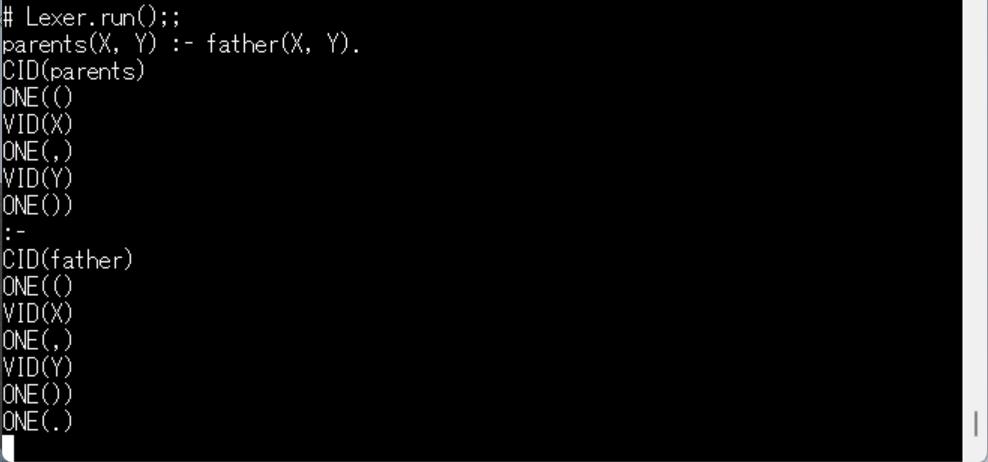
\includegraphics[scale = 0.6]{lexer_run.png}
\end{figure}

\section{問題2}
\subsection{問題内容}
与えられた文法において、左再帰の形をしたtermsとargsを右再帰に変換する。
\subsection{右再帰への変換}
\subsubsection{変換前}
terms \rightarrow \ term\par
terms \rightarrow \ terms "," term\par
args \rightarrow \ expr\par
args \rightarrow \ args "," expr\par


\subsubsection{変換後}
terms \rightarrow \ term terms'\par
terms' \rightarrow \ "," term terms'\par
terms' \rightarrow \ \par
args \rightarrow \ expr args'\par
args' \rightarrow \ "," expr args'\par
args' \rightarrow \par

\section{問題3}
\subsection{問題内容}
与えられた構文解析器プログラムの空欄を埋め、プログラムを完成させる。
\subsubsection{付加したコード}
\begin{lstlisting}[caption = to\_opt]
and to_opt() =
  match !tok with
    L.TO -> ( eat (L.TO); terms() )
  | _ -> ()
\end{lstlisting}

\begin{lstlisting}[caption = term]
and term() =
  match !tok with
    L.ONE '(' -> ( eat(L.ONE '('); term(); eat(L.ONE ')') )
  | _ -> predicate()
\end{lstlisting}

\begin{lstlisting}[caption = terms]
and terms() = ( term(); terms'() )
\end{lstlisting}

\begin{lstlisting}[caption = terms']
and terms'() =
  match !tok with
    L.ONE ',' -> ( eat(L.ONE ','); term(); terms'() )
  | _ -> ()
\end{lstlisting}

\begin{lstlisting}[caption = predicate]
and predicate() = ( eat(L.CID ""); eat(L.ONE '('); args(); eat(L.ONE ')') )
\end{lstlisting}

\begin{lstlisting}[caption = args]
and args() = ( expr(); args'() )
\end{lstlisting}

\begin{lstlisting}[caption = args']
and args'() = 
  match !tok with
    L.ONE ',' -> ( eat(L.ONE ','); expr(); args'() )
  | _ -> ()
\end{lstlisting}

\begin{lstlisting}[caption = expr]
and expr() =
  match !tok with
    L.ONE '(' -> ( eat(L.ONE '('); expr(); eat(L.ONE ')') )
  | L.ONE '[' -> ( eat(L.ONE '['); list(); eat(L.ONE ']') )
  | L.CID c -> ( eat(L.CID ""); tail_opt() )
  | L.VID v -> eat(L.VID "")
  | L.NUM n -> eat(L.NUM "")
  | _ -> error()
\end{lstlisting}

\begin{lstlisting}[caption = tail\_opt]
and tail_opt() =
  match !tok with
    L.ONE '(' -> ( eat(L.ONE '('); args(); eat(L.ONE ')') )
  | _ -> ()
\end{lstlisting}

\begin{lstlisting}[caption = id]
and id() =
  match !tok with
    L.CID c -> eat(L.CID "")
  | L.VID v -> eat(L.VID "")
  | L.NUM n -> eat(L.NUM "")
  | _ -> error()
\end{lstlisting}

\section{問題4}
\subsection{問題内容}
isono.plを用いて構文解析器の振る舞いを確認する。
\subsection{runの振る舞い}
\begin{figure}[htbp]
  \centering
  \caption{open isono.を実行したときのrunの振る舞い}
  \label{fig:run_isono}
  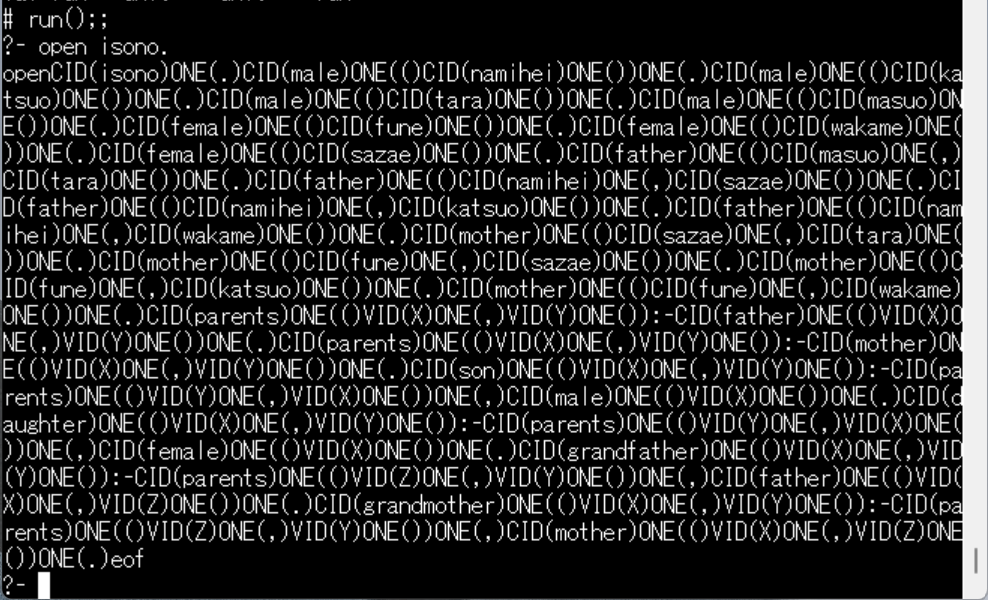
\includegraphics[scale = 0.6]{parser_run.png}
\end{figure}

\section{問題5}
\subsection{問題内容}
述語を「,」で区切り、複数の述語を入力できるようにプログラムを修正する。

\subsection{修正点}
Parserモジュールのcommand関数において、term \rightarrow \ termsとすればよい。


\begin{lstlisting}[caption = commandの修正]
(*修正前*)
and command() = 
  match !tok with
    L.QUIT -> exit 0
  | L.OPEN -> 
    (eat(L.OPEN);
    match !tok with
      L.CID s -> 
        eat(L.CID ""); 
        check (L.ONE '.');
        L._ISTREAM := open_in (s^".pl");
        advance(); 
        clauses(); 
        close_in (!L._ISTREAM)
    | _ -> error())
  | _ -> ( term(); check(L.ONE '.') )

(*修正後*)
and command() = 
  match !tok with
    L.QUIT -> exit 0
  | L.OPEN -> 
    (eat(L.OPEN);
    match !tok with
      L.CID s -> 
        eat(L.CID ""); 
        check (L.ONE '.');
        L._ISTREAM := open_in (s^".pl");
        advance(); 
        clauses(); 
        close_in (!L._ISTREAM)
    | _ -> error())
  | _ -> ( terms(); check(L.ONE '.') )
\end{lstlisting}


\subsection{動作確認}
\begin{figure}[ht]
  \centering
  \caption{runの複数の質問に対する実行結果}
  \label{fig:run_kamma}
  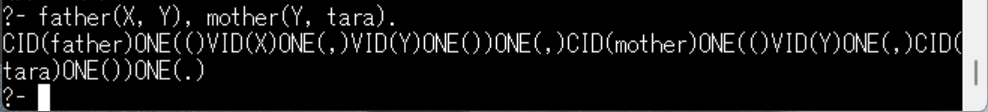
\includegraphics[scale = 0.6]{run_komma.png}
\end{figure}

\section{問題6}
\subsection{問題内容}
文法中にエラーが生じた際に、エラーが生じた個所の行番号を含む
エラーメッセージを印字するようにプログラムを修正する。
\subsection{修正点}
Lexerモジュール中に改行を読み込むたびに内部のカウントが1増える
変数line\_countを宣言する。Parserモジュールのcommand関数において、
try\dots with関数によりSyntax\_errorを検出し、printfを用いて
L.line\_countとともにエラーメッセージを印字する。
\begin{lstlisting}[caption = エラーメッセージ印字 修正点]
(*修正前*)
...
| OPEN 
| EOF 
| ONE of char

module P = Printf

let print_token tk =
...
and gettoken () =
  try
    let token = native_token () in
      match token with
        ONE ' ' -> gettoken ()
      | ONE '\t' -> gettoken ()
      | ONE '\n' -> gettoken ()
      | _ -> token
  with End_of_file -> EOF
...
and command() = 
  match !tok with
    L.QUIT -> exit 0
  | L.OPEN -> 
    (eat(L.OPEN);
    match !tok with
      L.CID s -> 
        eat(L.CID ""); 
        check (L.ONE '.');
        L._ISTREAM := open_in (s^".pl");
        advance(); 
        clauses(); 
        close_in (!L._ISTREAM)
    | _ -> error())
  | _ -> ( terms(); check(L.ONE '.') )
...


(*修正後*)
...
| OPEN 
| EOF 
| ONE of char

let line_count = ref 1

module P = Printf

let print_token tk =
...
and gettoken () =
  try
    let token = native_token () in
      match token with
        ONE ' ' -> gettoken ()
      | ONE '\t' -> gettoken ()
      | ONE '\n' -> ( line_count := !line_count + 1; gettoken () )
      | _ -> token
  with End_of_file -> ( line_count := 1; EOF )
...
and command() = 
  try
    match !tok with
      L.QUIT -> exit 0
    | L.OPEN -> 
      (!L.line_count := 1;
      eat(L.OPEN);
      match !tok with
        L.CID s -> 
          eat(L.CID ""); 
          check (L.ONE '.');
          L._ISTREAM := open_in (s^".pl");
          advance(); 
          clauses(); 
          close_in (!L._ISTREAM)
      | _ -> error())
    | _ -> ( L.line_count := 1; terms(); check(L.ONE '.') )
  with Syntax_error -> Printf.printf "\nline%d: Syntax error" !L.line_count
\end{lstlisting}

\subsection{実行結果}
実行結果を確認するために、7行目に構文ミスのあるファイルisono\_wrong.pl(図\ref{fig:iw})
を用意して、open isono\_wrong.を実行した。
また、構文ミスのある質問についても振る舞いを確認した。
\begin{figure}[htbp]
  \centering
  \caption{isono\_wrong.plの内容}
  \label{fig:iw}
  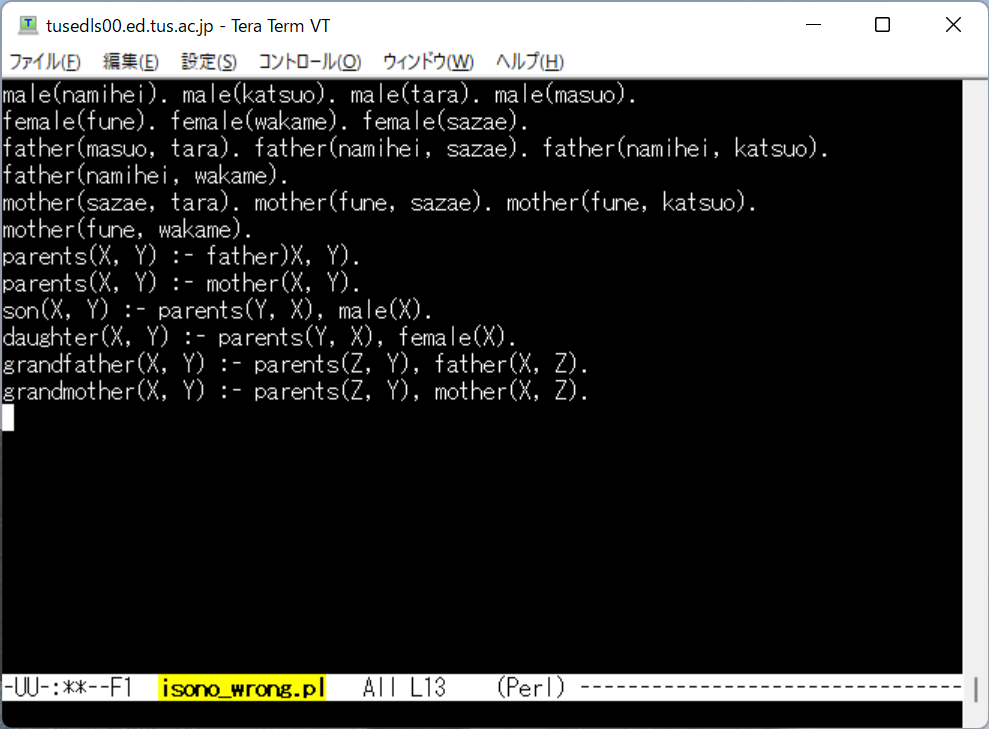
\includegraphics[scale = 0.6]{isono_wrong.png}
\end{figure}

\begin{figure}[htbp]
  \centering
  \caption{open isono\_wrong.の実行}
  \label{fig:run_wrong}
  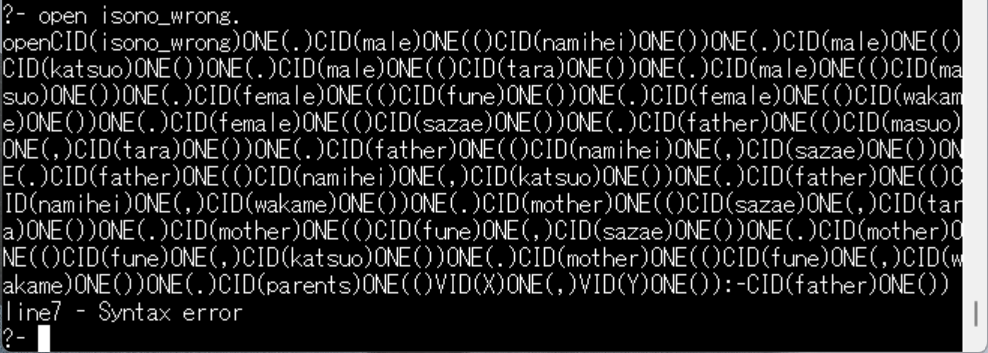
\includegraphics[scale = 0.6]{run_isono_wrong.png}
\end{figure}

\begin{figure}[htbp]
  \centering
  \caption{ミスのある質問の実行}
  \label{fig:run_wrong_q}
  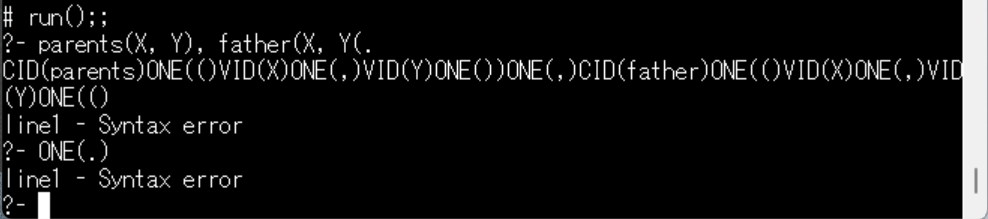
\includegraphics[scale = 0.6]{run_wrongcode.png}
\end{figure}


\subsection{考察}
図\ref{fig:run_wrong_q}を見ると、構文ミスのある箇所を受け取り、エラーメッセージを印字しているが、
その下では残ったピリオドも検出してエラーメッセージを印字してしまっている。
そこで、これを防ぐための方法を考えた。
それは、printfによるエラーメッセージの印字の後にraiseを用いることで、runを強制終了する方法だ。
これにより残った文章を検知して余分にエラーメッセージを印字してしまうことは無くなる。
しかし、エラーが起きるたびrunが終了してしまい、再びrunを起動する手間が発生してしまう。
よって、runの利用の仕方により、図\ref{fig:run_wrong_q}で示した方法と考察で示した
方法を使い分けるべきだと考える。

\section{問題7}
\subsection{問題内容}
算術式を記述できるように生成規則とプログラムを修正する。
\subsection{生成規則の修正}
問題文において算術式の記述に必要なarithmexpからなる生成規則が与えられているが、
左再帰が存在するため右再帰の形に変換する。
\subsubsection{変換前}
expr \rightarrow \  arithmexp\par
arithmexp \rightarrow \  arithmexp "+" arithmterm\par
arithmexp \rightarrow \  arithmexp "-" arithmterm\par
arithmexp \rightarrow \  arithmterm\par
arithmterm \rightarrow \  arithmterm "*" arithmfactor\par
arithmterm \rightarrow \  arithmterm "/" arithmfactor\par
arithmterm \rightarrow \  arithmfactor\par
arithmfactor \rightarrow \  "(" arithmexp ")"\par
arithmfactor \rightarrow \  "-" arithmexp\par
arithmfactor \rightarrow \  "[" list "]"\par
arithmfactor \rightarrow \  CID tail opt\par
arithmfactor \rightarrow \  VID\par
arithmfactor \rightarrow \  NUM\par

\subsubsection{変換後}
expr \rightarrow \  arithmexp\par
arithmexp \rightarrow \  arithmterm arithmexp'\par
arithmexp' \rightarrow \  "+" arithmterm arithmexp'\par
arithmexp' \rightarrow \  "-" arithmterm arithmexp'\par
arithmexp' \rightarrow \  \par
arithmterm \rightarrow \  arithmfactor arithmterm'\par
arithmterm' \rightarrow \   "*" arithmfactor arithmterm'\par
arithmterm' \rightarrow \   "/" arithmfactor arithmterm'\par
arithmterm' \rightarrow \  \par
arithmfactor \rightarrow \  "(" arithmexp ")"\par
arithmfactor \rightarrow \  "-" arithmexp\par
arithmfactor \rightarrow \  "[" list "]"\par
arithmfactor \rightarrow \  CID tail opt\par
arithmfactor \rightarrow \  VID\par
arithmfactor \rightarrow \  NUM\par

\subsection{修正したコード}
\begin{lstlisting}[caption = 算術式 修正点]
(*修正前*)
...
and expr() =
  match !tok with
    L.ONE '(' -> ( eat(L.ONE '('); expr(); eat(L.ONE ')') )
  | L.ONE '[' -> ( eat(L.ONE '['); list(); eat(L.ONE ']') )
  | L.CID c -> ( eat(L.CID ""); tail_opt() )
  | L.VID v -> eat(L.VID "")
  | L.NUM n -> eat(L.NUM "")
  | _ -> error()
...


(*修正後*)
...
and expr() = arithmexp()

and arithmexp() = ( arithmterm(); arithmexp'() )

and arithmexp'() =
  match !tok with
      L.ONE '+' -> ( eat(L.ONE '+'); arithmterm(); arithmexp'() )
    | L.ONE '-' -> ( eat(L.ONE '-'); arithmterm(); arithmexp'() ) 
    | _ -> ()

and arithmterm() = ( arithmfactor(); arithmterm' )

and arithmterm'() = 
  match !tok with 
      L.ONE '*' -> ( eat(L.ONE '*'); arithmfactor(); arithmterm'() )
    | L.ONE '/' -> ( eat(L.ONE '/'); arithmfactor(); arithmterm'() )
    | _ -> ()

and arithmfactor() = 
  match !tok with 
      L.ONE '(' -> ( eat(L.ONE '('); expr(); eat(L.ONE ')') )
    | L.ONE '[' -> ( eat(L.ONE '['); list(); eat(L.ONE ']') )
    | L.CID c -> ( eat(L.CID ""); tail_opt() )
    | L.VID v -> eat(L.VID "")
    | L.NUM n -> eat(L.NUM "")
    | _ -> error()
...
\end{lstlisting}

\section{問題8}
\subsection{問題内容}
変数への代入を記述できるようにプログラムを修正する。

\subsection{修正したコード}
\begin{lstlisting}[caption = 代入 修正点]
(*修正前*)
...
and term() =
  match !tok with
    L.ONE '(' -> ( eat(L.ONE '('); term(); eat(L.ONE ')') )
  | _ -> predicate()
...

(*修正後*)
...
and term() =
  match !tok with
    L.ONE '(' -> ( eat(L.ONE '('); term(); eat(L.ONE ')') )
  | L.VID _ -> ( eat(L.VID); eat(L.IS); arithmexp() )
  | _ -> predicate()
...

\end{lstlisting}


\end{document}